The eigenvector associated with $\lambda_1 = 2$ is $\boldsymbol{v}_1 = \begin{bmatrix}1 \\ 0\end{bmatrix}$ and the eigenvector associated with $\lambda_2 = -3$ is $\boldsymbol{v}_2 = \begin{bmatrix}0 \\ 1\end{bmatrix}$. Plot $\boldsymbol{v}_1$, $\boldsymbol{v}_2$, $\boldsymbol{Av}_1$, and $\boldsymbol{Av}_2$. What is the difference between a negative and positive eigenvalue?

\begin{solution} \
    \begin{center}
        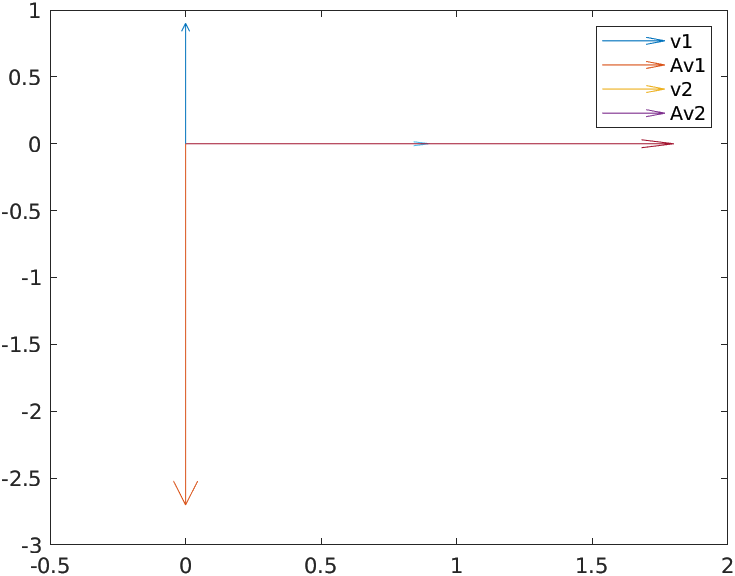
\includegraphics[width=0.6\textwidth]{img/e1p2.png}
    \end{center}

    A negative eigenvalue inverts the direction of the transformed vector.
\end{solution}